\documentclass[a4paper,11pt]{article}

\usepackage[
    a4paper,
    top=2.54cm,
    bottom=2.54cm,
    left=2.54cm,
    right=2.54cm
]{geometry}

\usepackage{xcolor}
\usepackage{tcolorbox}
\usepackage{enumitem}
\usepackage{hyperref}
\usepackage{titlesec}
\usepackage{booktabs}
\usepackage{tabularx}
\usepackage{array}

\setlist[itemize]{noitemsep, topsep=2pt}
\setlist[enumerate]{noitemsep, topsep=2pt}

\titleformat{\section}
    {\large\bfseries}{\thesection.}{0.5em}{}

\titleformat{\subsection}
    {\normalsize\bfseries}{\thesubsection.}{0.5em}{}

% Placeholder for values to be filled in by students.
\newcommand{\blank}[1][1.2cm]{\rule{#1}{0.4pt}}

\usepackage{graphicx}

\begin{document}

\begin{tcolorbox}[
    colback=white,
    colframe=black,
    width=\textwidth,
    arc=3mm,
    boxrule=1pt
]
\begin{center}
    \Large \textbf{Efficient Computing for Artificial Intelligence}\\[3pt]
    \large \textbf{Homework 1}\\[5pt]
    \textbf{\colorbox{yellow!30}{DUE DATE: 2 Dec (h23:59)}}\\[8pt]
\end{center}

\textbf{Submission Instructions:}\\[3pt]

Each group must send an e-mail to
\texttt{daniele.jahier@polito.it}, with
\texttt{valentino.peluso@polito.it} in CC.
Use the subject
\textbf{ECAI27 Group37}, replacing \texttt{N} with
the group ID.\\[3pt]

Attach a single ZIP archive named
\textbf{HW1\_Group37.zip}, containing:
\begin{enumerate}
    \item The code deliverables specified in each exercise.
    \item The PDF report.
\end{enumerate}

Late submissions or submissions that do not comply with these
instructions will be \textbf{automatically discarded}.
\end{tcolorbox}

\twocolumn[
\begin{@twocolumnfalse}
\begin{center}
\Large \textbf{HW1 – Group37}\\
\normalsize (Replace \texttt{N} with your group ID)\\

\begin{tabular}{lll}
\textbf{Surname Name} (s\texttt{XXXXXX}) & \textbf{Surname Name} (s\texttt{XXXXXX}) & \textbf{Surname Name} (s\texttt{XXXXXX}) \\
\end{tabular}
\end{center}
\end{@twocolumnfalse}
]

\section*{Results}

Complete the table with the operational intensity (OI), median latency,
and standard deviation of latency for each kernel.

\begin{itemize}
    \item \textbf{Operational intensity:}
    Report the ideal OI in FLOP/byte, assuming a single-level memory
    hierarchy and an infinite number of registers. 
    \item \textbf{Latency:}
    Report the median and standard deviation of the samples in milliseconds (ms), rounded
    to one decimal digit.
\end{itemize}

\begin{center}
\renewcommand{\arraystretch}{1.25}
\begin{tabularx}{\textwidth}{
    @{}
    >{\raggedright\arraybackslash}X
    >{\centering\arraybackslash}p{2.0cm}
    >{\centering\arraybackslash}p{2.6cm}
    >{\centering\arraybackslash}p{2.6cm}
    @{}
}
\toprule
Kernel
& OI (FLOP/byte)
& Median latency (ms)
& Std. latency (ms) \\
\midrule
% BEGIN RESULTS (filled by: python3 analysis/analyze.py ... --report <this file>)
Dense scalar & 42.7 & 563.1 & 14.5 \\
Dense tiled with NEON and OpenMP & 42.7 & 83.5 & 3.7 \\
Sparse scalar & 20.9 & 98.1 & 0.3 \\
Sparse NEON & 20.9 & 34.2 & 2.4 \\
Sparse tiled & 20.9 & 26.4 & 0.0 \\
Sparse OpenMP (2 threads) & 20.9 & 47.6 & 0.1 \\
Sparse OpenMP (4 threads) & 20.9 & 24.0 & 0.3 \\
Sparse Combined (2 threads) & 20.9 & 13.4 & 0.4 \\
Sparse Combined (4 threads) & 20.9 & 6.6 & 0.1 \\
% END RESULTS
\bottomrule
\end{tabularx}
\end{center}

\subsection*{Operational intensity}
Ideal OI = FLOP / compulsory bytes (FP32 values and \texttt{uint32}
indices, each moved once). $M=128$, $K=N=512$, $nnzb=4096$.
\begin{itemize}
    \item \textbf{Dense:} $2MKN = 67{,}108{,}864$ FLOP;
    $4(MK+KN+MN) = 1{,}572{,}864$ B $\Rightarrow$ \textbf{42.7 FLOP/B}.
    \item \textbf{Sparse:} $2\cdot16\,M\,nnzb = 16{,}777{,}216$ FLOP
    ($4\times$ fewer). Bytes: $A$ $4MK$ + values $4\cdot16\,nnzb$ +
    \texttt{block\_row\_idx} $4\,nnzb$ + \texttt{block\_col\_ptr}
    $4(N/4+1)$ + $C$ $4MN$ $= 803{,}332$ B $\Rightarrow$
    \textbf{20.9 FLOP/B}.
\end{itemize}
All sparse variants share the same ideal OI: tiling, NEON and OpenMP
change the \emph{achieved} traffic and parallelism, not the algorithmic
FLOP/byte ratio.

\IfFileExists{analysis/latency.png}{%
\begin{figure*}[p]
    \centering
    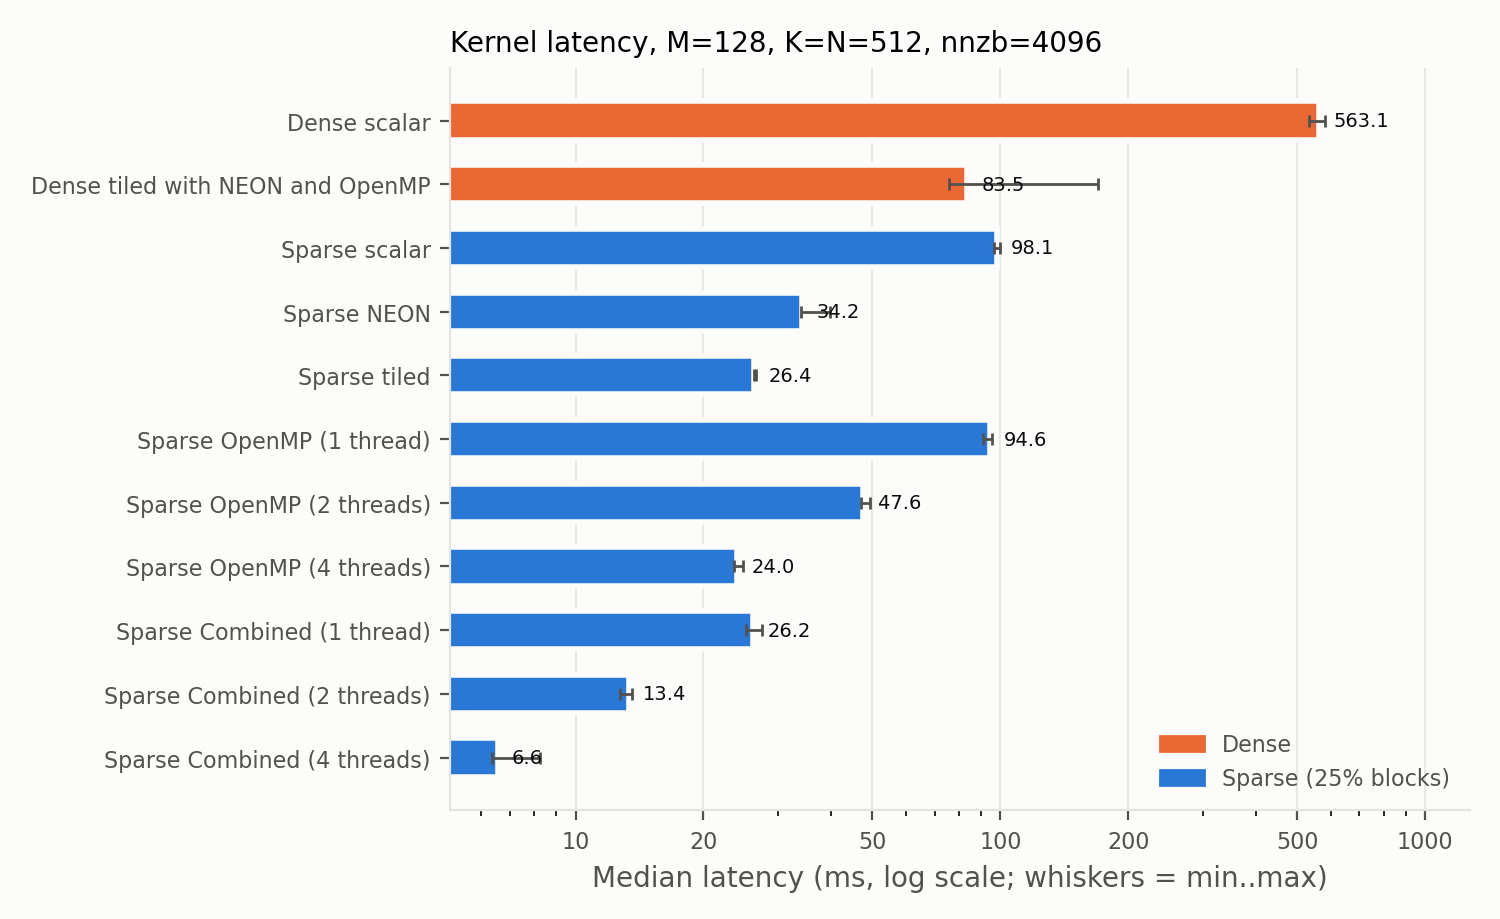
\includegraphics[width=0.49\textwidth]{analysis/latency.png}\hfill
    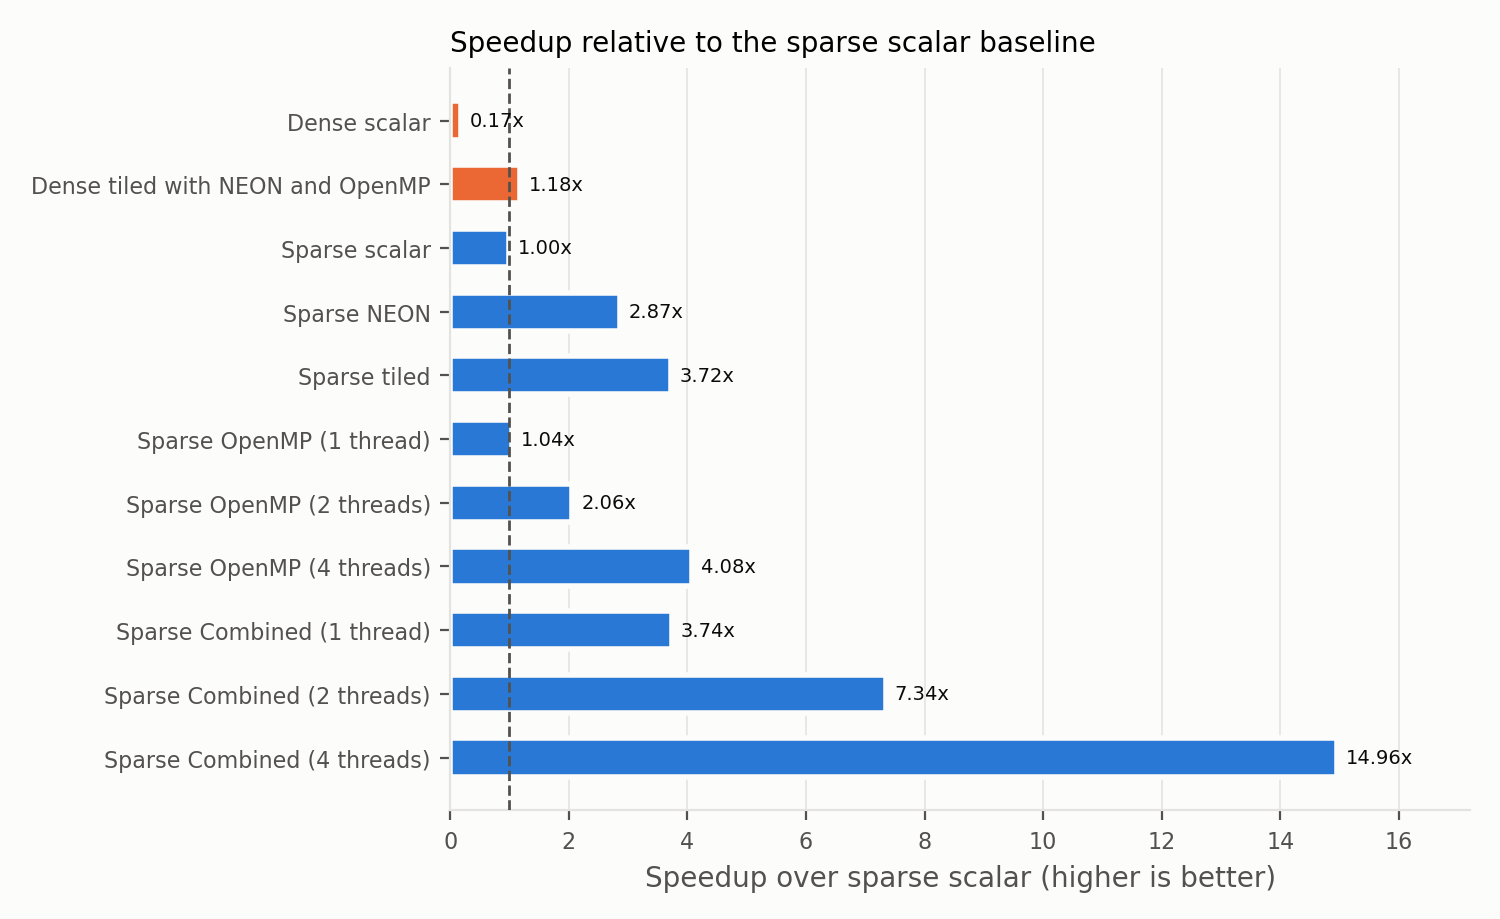
\includegraphics[width=0.49\textwidth]{analysis/speedup.png}\\[6pt]
    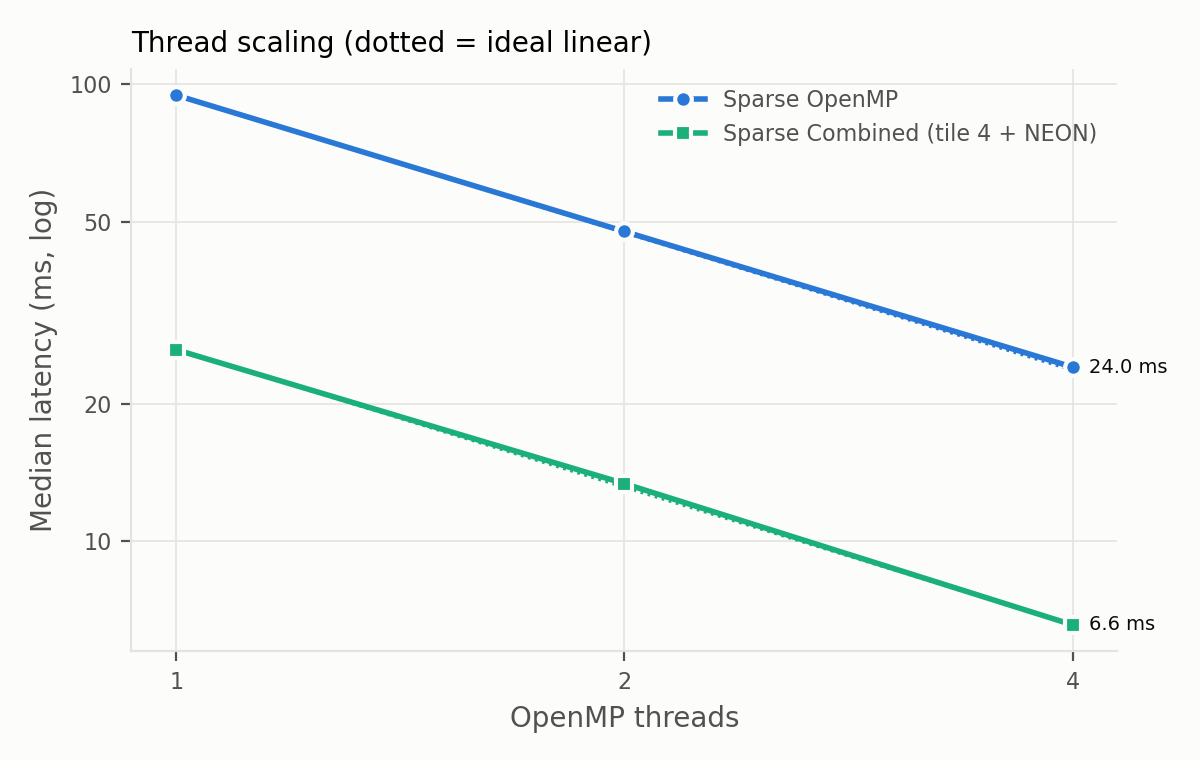
\includegraphics[width=0.6\textwidth]{analysis/thread_scaling.png}
    \caption{Raspberry Pi 4 measurements (median over runs): latency per
    kernel (whiskers = min..max of samples), speedup over sparse scalar,
    and OpenMP thread scaling.}
\end{figure*}}{}

\end{document}